\section{動的計画法(Dynamic Programming) 基本編}
動的計画法という競技プログラミングの最初の山となるアルゴリズムを紹介します。基本的な考え方はシンプルですが、さまざまな応用先がある重要なアルゴリズムです。
動的計画法の原則は以下のようなものです。

\begin{itemize}
  \item 与えられた問題を部分問題に分割する
  \item 部分問題の解を記録して再利用する
\end{itemize}

一度計算したものを記録して再び計算せずに利用することで効率的に計算を行うことができます。DPは慣れるまで難しいですが、慣れると非常に強力なアルゴリズムです。習うよりも慣れろということで、DPは具体的な問題を解きながら学ぶのが良いでしょう。

\subsection{フィボナッチ数列}
最も簡単なDPを紹介します。フィボナッチ数列を求める問題です。フィボナッチ数列は以下のように定義されます。

\begin{align*}
  F(0) &= 0 \\
  F(1) &= 1 \\
  F(n) &= F(n-1) + F(n-2) \quad (n \geq 2)
\end{align*}

この定義に基づいて、フィボナッチ数列を求めるプログラムを再帰関数を用いて実装すると以下のようになります。
\begin{lstlisting}[caption=再帰関数を用いたフィボナッチ数列の実装, frame=TRBL, label={rec_fib}]
def fib(n):
  if n == 0:
    return 0
  if n == 1:
    return 1
  return fib(n-1) + fib(n-2)
\end{lstlisting}

実装はシンプルですが、$n = 40$程度の大きさになると計算に時間がかかります。これは再帰関数を用いることで、同じ計算を何度も行っているためです。この問題を解決するために、DPを用いてフィボナッチ数列を求めるプログラムを実装します。

\begin{lstlisting}[caption=DPを用いたフィボナッチ数列の実装, frame=TRBL, label={dp_fib}]
def fib(n):
  dp = [0] * (n+1)
  dp[0] = 0
  dp[1] = 1
  for i in range(2, n+1):
    dp[i] = dp[i-1] + dp[i-2]
  return dp[n]
\end{lstlisting}

フィボナッチ数列の例を通じて、漸化式の計算を効率的に行うためにDPを用いることができることがわかりました。

\subsection{最大値問題}
次のDPの例題として、最大値問題を紹介します。最大値問題は、与えられた数列の中からいくつかの数を選んで総和を最大化する問題です。例えば、数列$[1, 2, 3, 4, 5]$が与えられたとき、この数列の中からいくつかの数を選んで総和を最大化する問題を考えます。
配列の中の正の数をすべて足せばいいですが、今回はDPを用いて解いてみます。ナイーブな実装では配列の要素を選ぶか選ばないかの$O(2^n)$の計算量になります。

DPには2つの方針としてメモ化再帰と漸化式があります。メモ化再帰は再帰関数を用いて大きい問題を分割する方法で、漸化式は小さい問題から順に解いていき大きい問題を解くための漸化式を求める方法です。

\subsubsection{メモ化再帰}
メモ化再帰を用いて最大値問題を解くプログラムを実装します。メモ化再帰は再帰関数を用いて計算を行い、計算結果を記録して再利用する方法です。以下にメモ化再帰を用いた最大値問題のプログラムを示します。
メモ化再帰の実装では、戻り値でメモした値を返すようにプログラムを書くことがポイントです。再帰をnから始めて
徐々に小さい問題に分割していくことで、最終的に大きい問題を解くことができます。

\begin{lstlisting}[caption=メモ化再帰を用いた最大値問題の実装, frame=TRBL, label={memo_max}]
def max_sum(A: list[int], memo: dict[int, int],limit: int):
  if limit < 0:
      return 0
  
  if limit in memo:
      return memo[limit]
  
  choose_current = A[limit] + max_sum(A, memo, limit - 1)
  skip_current = max_sum(A, memo, limit - 1)
  
  memo[limit] = max(choose_current, skip_current)
  return memo[limit]
\end{lstlisting}

\subsubsection{漸化式}
漸化式はメモ化再帰とは異なり、小さい問題から順に解いていき大きい問題を解くための漸化式を求める方法です。
最大値問題ではindex($\leq n - 1$)は直前の値に足すか足さないかの2通りがあるため、漸化式は以下のようになります。

\begin{align*}
  dp[i] = \max(dp[i-1] + A[i], dp[i-1])
\end{align*}

この漸化式を用いて最大値問題を解くプログラムを実装します。

\begin{lstlisting}[caption=漸化式を用いた最大値問題の実装, frame=TRBL, label={dp_max}]
def max_sum(A: list[int]) -> int:
    dp = [0] * len(A)
    # 初期化
    dp[0] = max(A[0], 0)
    
    for index, a in enumerate(A, 1):
        dp[index] = max(dp[index - 1], dp[index - 1] + A[index])
    
    return dp[len(A) - 1]
\end{lstlisting}

これで基本のDPの考え方は理解できたと思います。問題1を解いてみましょう。EDPCの基本問題です。メモ化再帰と漸化式の両方で
解いてみてください。

\subsection{コイン問題}
以下の問題を考えてみましょう。今までのDPの考え方に加えて少し応用を加えた問題です。後で扱うナップサック問題の基本となる問題です。

\begin{problem}
  $m$種類のコインがあり、それぞれのコインは無限にあるとする。コインの価値がそれぞれ$c_1, c_2, \ldots, c_m$であるとき、合計金額が$n$円になるようにコインを選ぶ方法の最小枚数を求めよ。
\end{problem}

価値が大きい方から選ぶという貪欲法では最適解が求められないため、DPを用いて解く必要があります。こちらの問題もメモ化再帰と漸化式の両方で解いてみます。

\begin{lstlisting}[caption=メモ化再帰を用いたコイン問題の実装, frame=TRBL, label={memo_coin}]
def minimum_coin_counts(coins: list[int], memo: dict[int], limit: int) -> int:
  if limit in coins:
      memo[limit] = 1
      return 1
  
  if limit in memo:
      return memo[limit]
  if limit - coins[0] > 0:
      memo[limit] = minimum_coin_counts(coins, memo, limit - coins[0]) + 1    
  
  for coin in coins:
      if limit - coin > 0:
          memo[limit] = min(minimum_coin_counts(coins, memo, limit - coin) + 1, memo[limit])

  return memo[limit]
\end{lstlisting}

\begin{lstlisting}[caption=漸化式を用いたコイン問題の実装, frame=TRBL, label={dp_coin}]
def minimum_coin_count(m: int, n: int, coins: list[int]) -> int:
  # dp table
  dp = [1 << 60] * (n + 1)
  # 初期化
  dp[0] = 0
  
  for i in range(1, n + 1):
      for coin in coins:
          if i - coin >= 0:
              dp[i] = min(dp[i], dp[i - coin] + 1)
  
  return dp[n]
\end{lstlisting}

メモ化再帰と漸化式の両方で、「ずらした値 + コスト」(dp[i - coin] + 1)という形で解いていることがわかります。動的計画法において
前のどの結果を使うのかを考えることが重要です。続くナップサック問題でも同様の考え方が使われます。

メモ化再帰と漸化式どちらが考えやすいかは人それぞれですが、漸化式の方が実装が簡単であることが多いです。

\subsection{ナップサック問題}
ナップサック問題はDPの中でも有名な問題です。ナップサック問題は以下のような設定の問題です。

\begin{problem}
  重さが$w_1, w_2, \ldots, w_n$で価値が$v_1, v_2, \ldots, v_n$である$n$個の品物があり、重さの総和が$W$を超えないようにナップサックに詰め込むとき、価値の総和の最大値を求めよ。
\end{problem}

各荷物について品物を入れるか入れないかの2通りがあるため、0/1ナップサック問題と呼ばれます。先ほどまでの問題とは違って価値と重さという2つの基準がある問題です。dpテーブルが2次元の配列になるため、実装が少し複雑になります。
ナップサック問題はメモ化再帰と漸化式の両方で解いてみましょう。

\begin{lstlisting}[caption=メモ化再帰を用いたナップサック問題の実装, frame=TRBL, label={memo_knapsack}]
def recursive_knapsack(item_limit: int, weight_limit: int, memo: dict[tuple[int, int], int], items: list[tuple[int, int]]) -> int:
    if (item_limit, weight_limit) in memo:
        return memo[(item_limit, weight_limit)]
    
    if item_limit == 0 or weight_limit == 0:
        return 0
    
    value, weight = items[item_limit]
    
    not_taken = recursive_knapsack(item_limit - 1, weight_limit, memo, items)
    
    taken = 0
    if weight_limit - weight >= 0:
        taken = value + recursive_knapsack(item_limit - 1, weight_limit - weight, memo, items)
    
    memo[(item_limit, weight_limit)] = max(not_taken, taken)
    
    return memo[(item_limit, weight_limit)]

def main():
    n, w = map(int, input().split())
    items = [(0, 0)]  
    for i in range(n):
        value, weight = map(int, input().split())
        items.append((value, weight))
    
    memo = dict()
    
    ans = recursive_knapsack(n, w, memo, items)
    
    print(ans)

if __name__ == "__main__":
    main()
\end{lstlisting}

\begin{lstlisting}[caption=漸化式を用いたナップサック問題の実装, frame=TRBL, label={dp_knapsack}]
def knapsack(n: int, w: int, items: list[tuple[int, int]]) -> int:
    dp = [[0] * (w + 1) for _ in range(n + 1)]
    
    for i in range(1, n + 1):
        value, weight = items[i]
        for j in range(1, w + 1):
            if j - weight >= 0:
                dp[i][j] = max(dp[i - 1][j], dp[i - 1][j - weight] + value)
            else:
                dp[i][j] = dp[i - 1][j]
    
    return dp[n][w]
\end{lstlisting}

\subsection{問題}
\textbf{問題1} EDPC A - Frog 1\\
\textbf{問題2} AtCoder Beginner Contest 032 ナップサック問題\\  
上で扱ったナップサック問題とは少しだけ設定が異なる問題です。\\

\textbf{参考}
\begin{itemize}
  \item \url{https://dai1741.github.io/maximum-algo-2012/docs/dynamic-programming/}
  \item \url{}
\end{itemize}

\section{動的計画法 応用編}
動的計画法は幅広い応用先があります。ここでは、動的計画法の応用例を紹介します。
\subsection{レーベンシュタイン距離}
レーベンシュタイン距離とは、ある文字列Aと別の文字列Bの類似度を計算するための指標の1つです。レーベンシュタイン距離は、文字列Aから文字列Bに変換するために必要な操作回数の最小回数を表します。操作は以下の3つがあります。

\begin{itemize}
  \item 挿入: 文字列Aに文字を挿入する
  \item 削除: 文字列Aから文字を削除する
  \item 置換: 文字列Aの文字を別の文字に置換する
\end{itemize}

例えば、kittenとsettingのレーベンシュタイン距離は3です。以下のように計算できます。

\begin{itemize}
  \item kitten $\to$ sitten (置換: $k \to s$)
  \item sitten $\to$ settin (置換: $i \to $e)
  \item settin $\to$ setting (挿入: $g$)
\end{itemize}

漸化式タイプの動的計画法を使ってレーベンシュタイン距離を考えてみましょう。簡単のために文字列A、Bはそれぞれabc, adcdとします。
dpテーブルの各セル(i, j)は文字列Aのi文字目までと文字列Bのj文字目までのレーベンシュタイン距離を表します。dpテーブルでの処理と
文字列操作の対応を考えましょう。

1列目と1行目は空文字列です。空文字列から文字列Aのi文字目までのレーベンシュタイン距離はiです。同様に空文字列から文字列Bのj文字目までのレーベンシュタイン距離はjです。dpテーブルは以下のようになります。

\begin{table}[h]
  \centering
  \begin{tabular}{|c|c|c|c|c|c|}
    \hline
    & "" & a & b & d  & c\\
    \hline
    "" & 0 & 1 & 2 & 3 & 4\\
    \hline
    a & 1 &  &  &  & \\
    \hline
    b & 2 &  &  &  & \\
    \hline
    c & 3 &  &  &  & \\
    \hline
  \end{tabular}
\end{table}

1列目を考えると、空文字列から文字列Bのi文字目までのレーベンシュタイン距離を表していますが、右への移動は\textbf{挿入}の操作を表しています。同様に1行目を考えると、文字列Aのi文字目から空文字列へのレーベンシュタイン距離を表しており、下への移動は\textbf{削除}の操作を表しています。
テーブルで斜めに進むことは、文字列操作においては\textbf{置換}または\textbf{何もしない}の操作を表しています。テーブル上で削除してから追加する(下に行ってから右に行く)という操作は、置換と等価です。
追加してから削除する(右に行ってから下に行く)という操作は、何もしないと等価です。よって、dpテーブルの更新は以下のようになります。

\begin{itemize}
  \item 追加: dp[i][j] = dp[i][j-1] + 1
  \item 削除: dp[i][j] = dp[i-1][j] + 1
  \item 置換: dp[i][j] = dp[i-1][j-1] + 1
  \item 何もしない: dp[i][j] = dp[i-1][j-1]
\end{itemize}

完成したdpテーブルは以下のようになります。

\begin{table}[h]
  \centering
  \begin{tabular}{|c|c|c|c|c|c|}
    \hline
    & "" & a & b & d  & c\\
    \hline
    "" & 0 & 1 & 2 & 3 & 4\\
    \hline
    a & 1 & 0 & 1 & 2 & 3\\
    \hline
    b & 2 & 1 & 1 & 2 & 3\\
    \hline
    c & 3 & 2 & 2 & 1 & 2\\
    \hline
  \end{tabular}
\end{table}

レーベンシュタイン距離の実装を漸化式を用いて実装してみましょう。

\begin{lstlisting}[caption=レーベンシュタイン距離の実装, frame=TRBL, label={levenshtein}]
def levenshtein(str1: str, str2: str) -> int:
  dp = [[0] * (len(str2) + 1) for _ in range(len(str1) + 1)]
  # 初期化
  for i in range(1, len(str2) + 1):
      dp[0][i] = i

  for i in range(1, len(str1) + 1):
      dp[i][0] = i
  
  # dpテーブル更新
  for i in range(1, len(str1) + 1):
      for j in range(1, len(str2) + 1):
          if str1[i - 1] == str2[j - 1]:
              dp[i][j] = min(dp[i][j - 1] + 1, dp[i - 1][j] + 1, dp[i - 1][j - 1])
          else:
              dp[i][j] = min(dp[i][j - 1] + 1, dp[i - 1][j] + 1, dp[i - 1][j - 1] + 1)
          
  return dp[len(str1)][len(str2)]
\end{lstlisting}

\subsection{動的時間伸縮法(Ddynamic Time Warping, DTW)}
2つの時系列データの類似度を計算するための手法です。DTWは時系列データの長さが異なる場合でも、2つの時系列データの類似度を計算することができ、弾性マッチング(Elastic Matching)とも呼ばれます。
時系列データ間の類似度を計算するにはユークリッド距離を使うこともできますが、それでは時系列データの類似度をうまく測れなかったり、時系列データの長さが異なる場合に対応できません。

\begin{center}
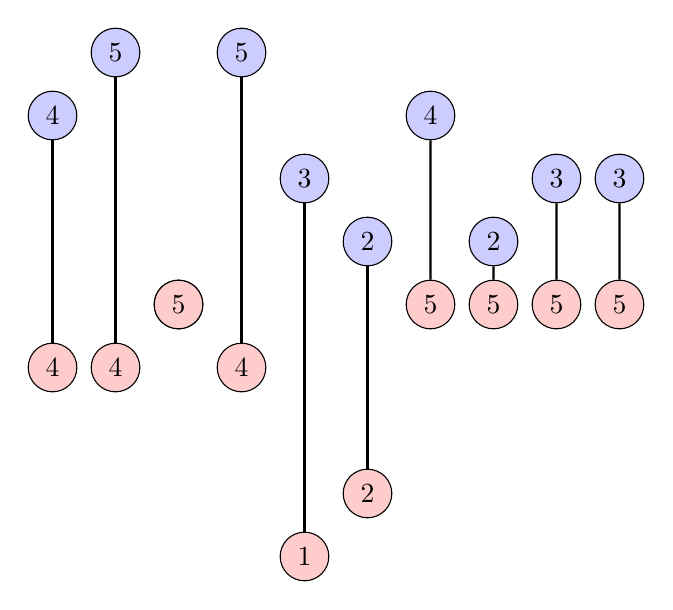
\begin{tikzpicture}[scale=0.8]
  \pgfmathsetseed{123}

  \foreach \i in {1,...,10} {
      \pgfmathtruncatemacro{\randomnum}{random(1,5)} 
      \node[circle, draw, fill=blue!20] (a\i) at (\i, \randomnum + 2) {\randomnum};
  }

  \foreach \i in {1,...,10} {
      \pgfmathtruncatemacro{\randomnum}{random(1,5)} 
      \node[circle, draw, fill=red!20] (b\i) at (\i, \randomnum - 2) {\randomnum}; 
  }

  \foreach \i in {1,...,10} {
      \draw[thick] (a\i) -- (b\i);
  }
\end{tikzpicture}
\end{center}

\vspace{0.5cm}

ユークリッド距離では同じ時間のデータの距離を計算しますが、DTWでは異なる時間のデータまで考慮して距離が最も小さくなるように計算します。DTWは以下のような特徴を持ちます。

\begin{itemize}
  \item 1つのデータにあるすべての要素は、少なくとも1つのデータの1つ以上の要素とペア組みされる
  \item ペア組は1対多の関係を持つことができる
  \item 1つの時系列データのある要素は、もう1つの時系列データの複数の要素とペア組みされることができる
\end{itemize}

ペア組する際の条件は以下のようになります。
1つ目の時系列データをX、2つ目の時系列データをYとします。Xのi番目の要素を$x_i$、Yのj番目の要素を$y_j$とします。すべての$i, j$に関して、X[i]とY[j]がペア組みされているとき、X[i]とY[j]のペア組みは以下の条件を満たします。
\begin{itemize}
  \item a[i + 1]以降の要素は、b[j]かb[j]以降の要素とペア組みされる
  \item b[j + 1]以降の要素は、a[i]かa[i]以降の要素とペア組みされる
\end{itemize}

これらはつまり、交差しないようにペア組みを行うということです。dpテーブルの作成をします。2つの時系列データa, bを考えたとき、dpテーブルのセル(i, j)はa[i]までの時系列データと
b[j]までの時系列データとの最小の距離を表します。dpテーブルの初期化は、片方の時系列データの長さが1のとき、もう一方の時系列データとそれぞれの距離を計算します。

a = [4, 1, 5, 2, 6], b = [3, 1, 4, 1, 5]の場合、dpテーブルは以下のように初期化します。

\vspace{0.5cm}

\begin{table}[h]
  \centering
  \begin{tabular}{c|c|c|c|c|c|}
    & b[0] & b[1] & b[2] & b[3] & b[4]\\
    \hline
    a[0]&  1 & 4 & 4 & 7  & 8\\
    \hline
    a[1]&  3 &  &  &   & \\
    \hline
    a[2]&  5 &  &  &  & \\
    \hline
    a[3]&  6 &  &  &   & \\
    \hline
    a[4]&  9 &  &  &   & \\
    \hline
  \end{tabular}
\end{table}

\vspace{0.5cm}

操作とdpテーブ上での動きの対応は以下のようになります。

\begin{itemize}
  \item a[i-1]とb[j]まではすでにペア組みが終わっていて、a[i]とb[j]をペアとする
  \item a[i]と[j-1]まではすでにペア組みが終わっていて、a[i]とb[j]をペアとする
  \item a[i-1]とb[j-1]まではすでにペア組みが終わっていて、a[i]とb[j]をペアとする
\end{itemize}

DTWの実装例は以下のようになります。
\begin{lstlisting}[caption=DTWの実装, frame=TRBL, label={dtw}]
def dist(x: int, y: int) -> int:
  return (x - y) ** 2

def dtw(a: list[int], b: list[int]) -> int:
  n, m = len(a), len(b)
  dp = [[0 for j in range(m)] for i in range(n)]
  
  for i in range(1, n):
      dp[i][0] = dp[i-1][0] + dist[a[i], b[0]]
  for i in range(1, m):
      dp[0][i] = dp[0][i - 1] + dist[a[0], b[i]]
  
  for i in range(1, n):
      for j in range(1, m):
          dp[i][j] = min(min(dp[i-1][j], dp[i][j - 1]), dp[i][j-1], dp[i - 1][j - 1]) + dist(a[i], b[j])
  
  return dp[n][m]
\end{lstlisting}